\Opensolutionfile{solutions}[ex]
\section*{Exercises}

\begin{enumialphparenastyle}

\begin{ex}
  Draw the complex numbers $z = 2+i$ and $w = -2+3i$ as points in the
  plane. Then use the geometric interpretation to find $z+w$,
  $z-w$, $zw$, $z^{-1}$, $\overline{z}$, and $\abs{z}$. 
\end{ex}

\begin{ex}
  Use the geometric interpretation to find a complex number $z$ such
  that $z^2 = i$. Can you find two such numbers?
  \begin{sol}
    Since $i$ has magnitude $1$ and argument $\pi/2$ (or
    $90^{\circ})$, the number $z$ must have magnitude $1$ and argument
    $\pi/4$. It therefore lies at $45^{\circ}$ on the unit circle. The
    solution is $z=\frac{1+i}{\sqrt{2}}$. A second solution is
    $-z=-\frac{1+i}{\sqrt{2}}$, whose argument is $-3\pi/4$ or
    $-135^{\circ}$. Note that if we double this angle, we get
    $-270^{\circ}$, which is the same as $+90^{\circ}$.
    \begin{equation*}
      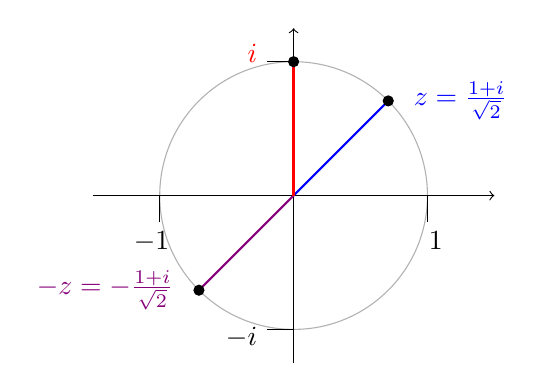
\begin{tikzpicture}[scale=1.7]
        \draw[black!30] (0,0) circle (1);
        \draw[->](-1.5,0) -- (1.5,0);
        \draw[->](0,-1.25) -- (0,1.25);
        \draw(0,-1) -- +(-0.2,0) node[left,yshift=-3pt] {$-i$};
        \draw(0,1) -- +(-0.2,0) node[left,yshift=3pt,red] {$i$};
        \draw(-1,0) -- +(0,-0.2) node[below,xshift=-3pt] {$-1$};
        \draw(1,0) -- +(0,-0.2) node[below,xshift=3pt] {$1$};
        \draw[thick, blue] (0,0) -- (45:1);
        \draw[thick, purple!70!blue] (0,0) -- (225:1);
        \draw[thick, red] (0,0) -- (90:1);
        \draw[fill, black] (45:1) circle [radius=1.06pt] node [right=2mm, blue] {$z = \frac{1+i}{\sqrt{2}}$};
        \draw[fill, black] (225:1) circle [radius=1.06pt] node [left=2mm, purple!70!blue] {$-z = -\frac{1+i}{\sqrt{2}}$};
        \draw[fill, black] (90:1) circle [radius=1.06pt];
      \end{tikzpicture}
    \end{equation*}
  \end{sol}
\end{ex}

\begin{ex}
  Use the geometric interpretation to find 3 different complex numbers
  $z$ such that $z^3 = -1$. Hint: these numbers will lie on the unit
  circle.
  \begin{sol}
    The three solutions can be found on the unit circle at
    $60^{\circ}$, $180^{\circ}$, and $300^{\circ}$. If we triple any
    of these angles, we get $180^{\circ}$ (up to multiples of $360^{\circ}$).
    Thus, the three cube roots of $-1$ are $z=-1$ and $z=0.5\pm\sqrt{0.75}\,i$.
    \begin{equation*}
      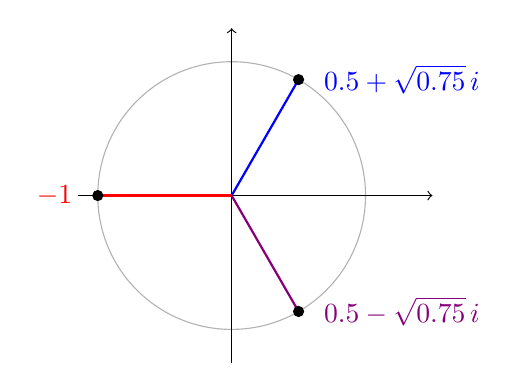
\begin{tikzpicture}[scale=1.7]
        \draw[black!30] (0,0) circle (1);
        \draw[->](-1.15,0) -- (1.5,0);
        \draw[->](0,-1.25) -- (0,1.25);
        \draw[thick, blue] (0,0) -- (60:1);
        \draw[thick, red] (0,0) -- (180:1);
        \draw[thick, purple!70!blue] (0,0) -- (300:1);
        \draw[fill, black] (60:1) circle [radius=1.06pt] node [right=2mm,blue] {$0.5+\sqrt{0.75}\,i$};
        \draw[fill, black] (180:1) circle [radius=1.06pt] node [left=2mm,red] {$-1$};
        \draw[fill, black] (300:1) circle [radius=1.06pt] node [right=2mm,purple!70!blue] {$0.5-\sqrt{0.75}\,i$};
      \end{tikzpicture}
    \end{equation*}
  \end{sol}
\end{ex}

\end{enumialphparenastyle}
